\documentclass{article}
\usepackage[utf8]{inputenc}
\usepackage{amssymb}
\usepackage{amsfonts}
\usepackage{amsmath}
\usepackage[utf8]{inputenc}
\usepackage[norsk]{babel}
\usepackage{lmodern}
\usepackage{float}
\usepackage{graphicx}
\DeclareGraphicsExtensions{.pdf,.png,.jpg}
\usepackage{latexsym}
\usepackage{hyperref}
\usepackage[euler]{textgreek}
\usepackage{stackengine}
\usepackage{pdfpages}
\usepackage{fixltx2e}
\hypersetup{pdfborder={0 0 0}}
\usepackage{pgfplots}
\pgfplotsset{compat=newest}
\pgfplotsset{plot coordinates/math parser=false}
\newlength\figureheight
\newlength\figurewidth
\usepackage[section]{placeins}%Sørger for at plots og andre floats holder seg til sin section.
\setlength\parindent{0pt}%Setter indent til 0



\title{Exercise 1 - TTK4130 Modeling and Simulation}
\author{Camilla Sterud}

\begin{document}

\maketitle

\newpage

\section{Problem 1}

\begin{align}
	Ni = \phi(\mathcal R_a + \mathcal R_c + \mathcal R_b + \mathcal R_r).\label{eq:Ni}\\ 
	\mathcal R_a = \frac{z}{A\mu_0}, \mathcal R_r = const. \label{eq:R_a} \\ 
	\mathcal R_c, \mathcal R_b << \mathcal R_r, \mathcal R_a. \label{eq:small}
\end{align}


\subsection{a}

\begin{equation}\label{eq:R_r}
	\mathcal R_r = \frac{z_0}{A\mu_0}, z_0 = const.
\end{equation}

Using Equation \ref{eq:Ni} together with the relations from equations \ref{eq:R_a} and \ref{eq:R_r} we get

\begin{equation*}
	Ni = \phi(\frac{z}{A\mu_0} + \mathcal R_c + \mathcal R_b + \frac{z_0}{A\mu_0}).
\end{equation*}

Since $\mathcal R_c$ and $\mathcal R_b$ are neligible (Equation \ref{eq:small}), the total magnetomotive force on the ball is

\begin{equation*}
	\underline{\underline{Ni = \frac{\phi}{A\mu_0}(z + z_0).}}
\end{equation*}

\subsection{b}

\begin{equation} \label{eq:induct}
	L(z) = \frac{N\phi}{i} = \frac{N^2A\mu_0}{z + z_0}.
\end{equation}

\begin{equation}\label{eq:magnF}
	F = \frac{i^2}{2}\frac{\partial L(z)}{\partial z}.
\end{equation}

Assume positive direction downwards and gravitational acceleration $g$.

\begin{align*}
	ma = \Sigma F\\
	m\ddot z = mg + F\\
	m\ddot z = mg + \frac{i^2}{2}N^2A\mu_0(z + z_0)^{-2}.
\end{align*}

\begin{equation}\label{eq:motion}
	\underline{\underline{\ddot z = g - \frac{1}{2m}i^2N^2A\mu_0(z+z_0)^{-2}}}
\end{equation}


\subsection{c}
Linearizing about $z_d$, $\dot z_d = 0$, $\ddot z_d = 0$.
\begin{align*}
	0 = g - \frac{1}{2m}i_d^2N^2A\mu_0(z_d+z_0)^{-2}\\
	i_d = \frac{1}{N}\sqrt{\frac{2mg}{A\mu_0}}(z_d + z_0)
\end{align*}

Equation \ref{eq:motion} we now call $f_1$. We define $z = z_d + \Delta z, i = i_d + \Delta i$ and thereby $\dot z = \Delta\dot z$. A Linearization of Equation \ref{eq:motion} around the point $z_d$ is then


	$\Delta\ddot z = \left. \frac{\partial f_1}{\partial \dot z} \right.\Bigg|_{\shortstack{\tiny $z = z_d$ \\ \tiny $\dot z = \dot z_d$ \\ \tiny $i = i_d$}} \Delta \dot z + \left. \frac{\partial f_1}{\partial z} \right.\Bigg|_{\shortstack{\tiny $z = z_d$ \\ \tiny $\dot z = \dot z_d$ \\ \tiny $i = i_d$}} \Delta z + \left. \frac{\partial f_1}{\partial i} \right.\Bigg|_{\shortstack{\tiny $z = z_d$ \\ \tiny $\dot z = \dot z_d$ \\ \tiny $i = i_d$}} \Delta i\\$

\begin{equation*}
	\Delta\ddot z = \frac{1}{m}i_d^2N^2A\mu_0(z_d+z_0)^{-3} \Delta z - \frac{1}{2m}i_dN^2A\mu_0(z_d+z_0)^{-2}\Delta i
\end{equation*}


\begin{equation*}
	\underline{\underline{\Delta \ddot z = \frac{2g}{z_d + z_0} \Delta z - \frac{N}{z_d + z_0}\sqrt{\frac{2gA\mu_0}{m}} \Delta i}}
\end{equation*}


\newpage
\section{Problem 2}

\subsection{b}

Natural signal-flow inputs are $T_i$ and $\omega_{i-1}$. The outputs should be $T_{i-1}$ and $\omega_i$. For natural energy-flow, inputs should be $T_{i-1}$ and $\omega{i-1}$, with $T_i$ and $\omega_i$ as outputs. 

\subsection{c}

\begin{figure}[!ht]
    \centering
    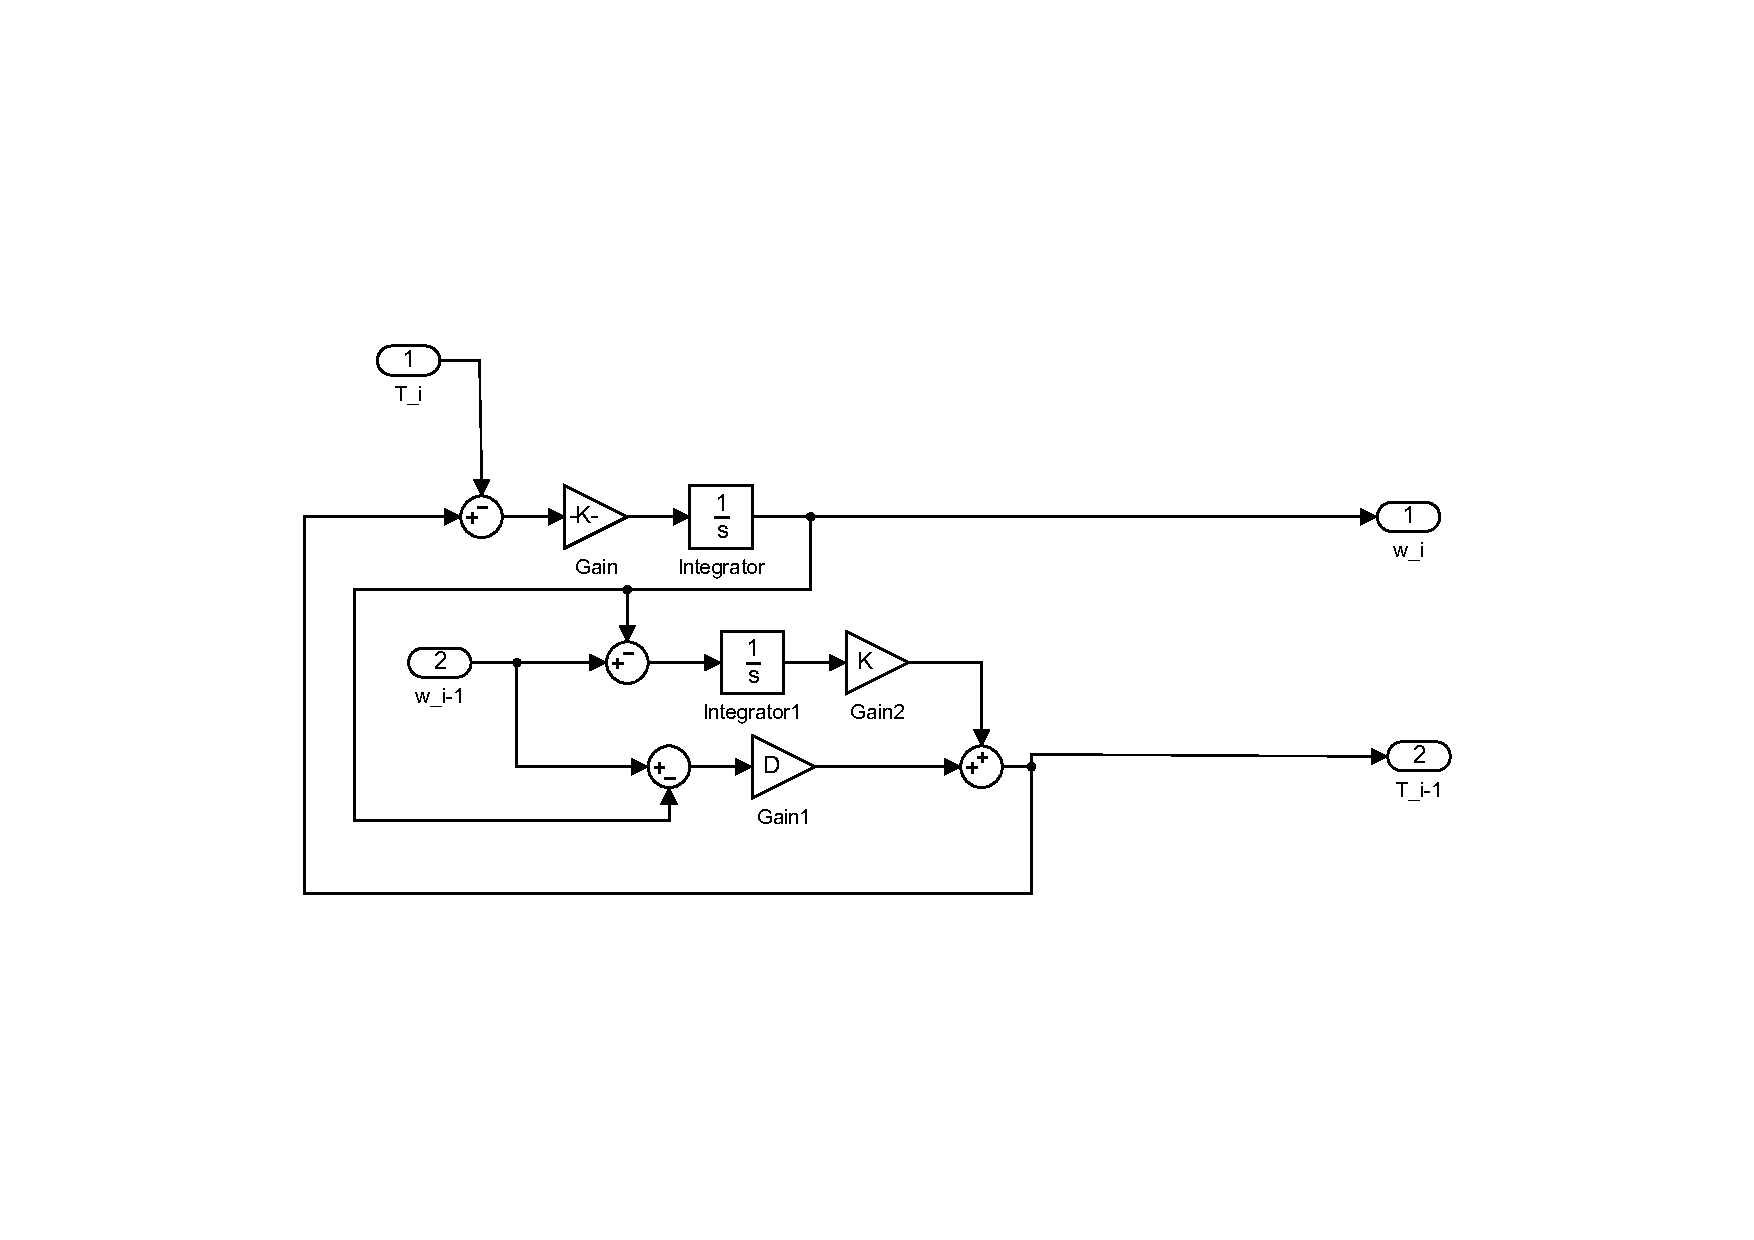
\includegraphics[width = \textwidth]{ex1_2_elasticload}
    \caption{The elastic load implemented in Simulink}
    \label{fig:elasticload} 
\end{figure}

\subsection{d}

\begin{figure}[!ht]
    \centering
    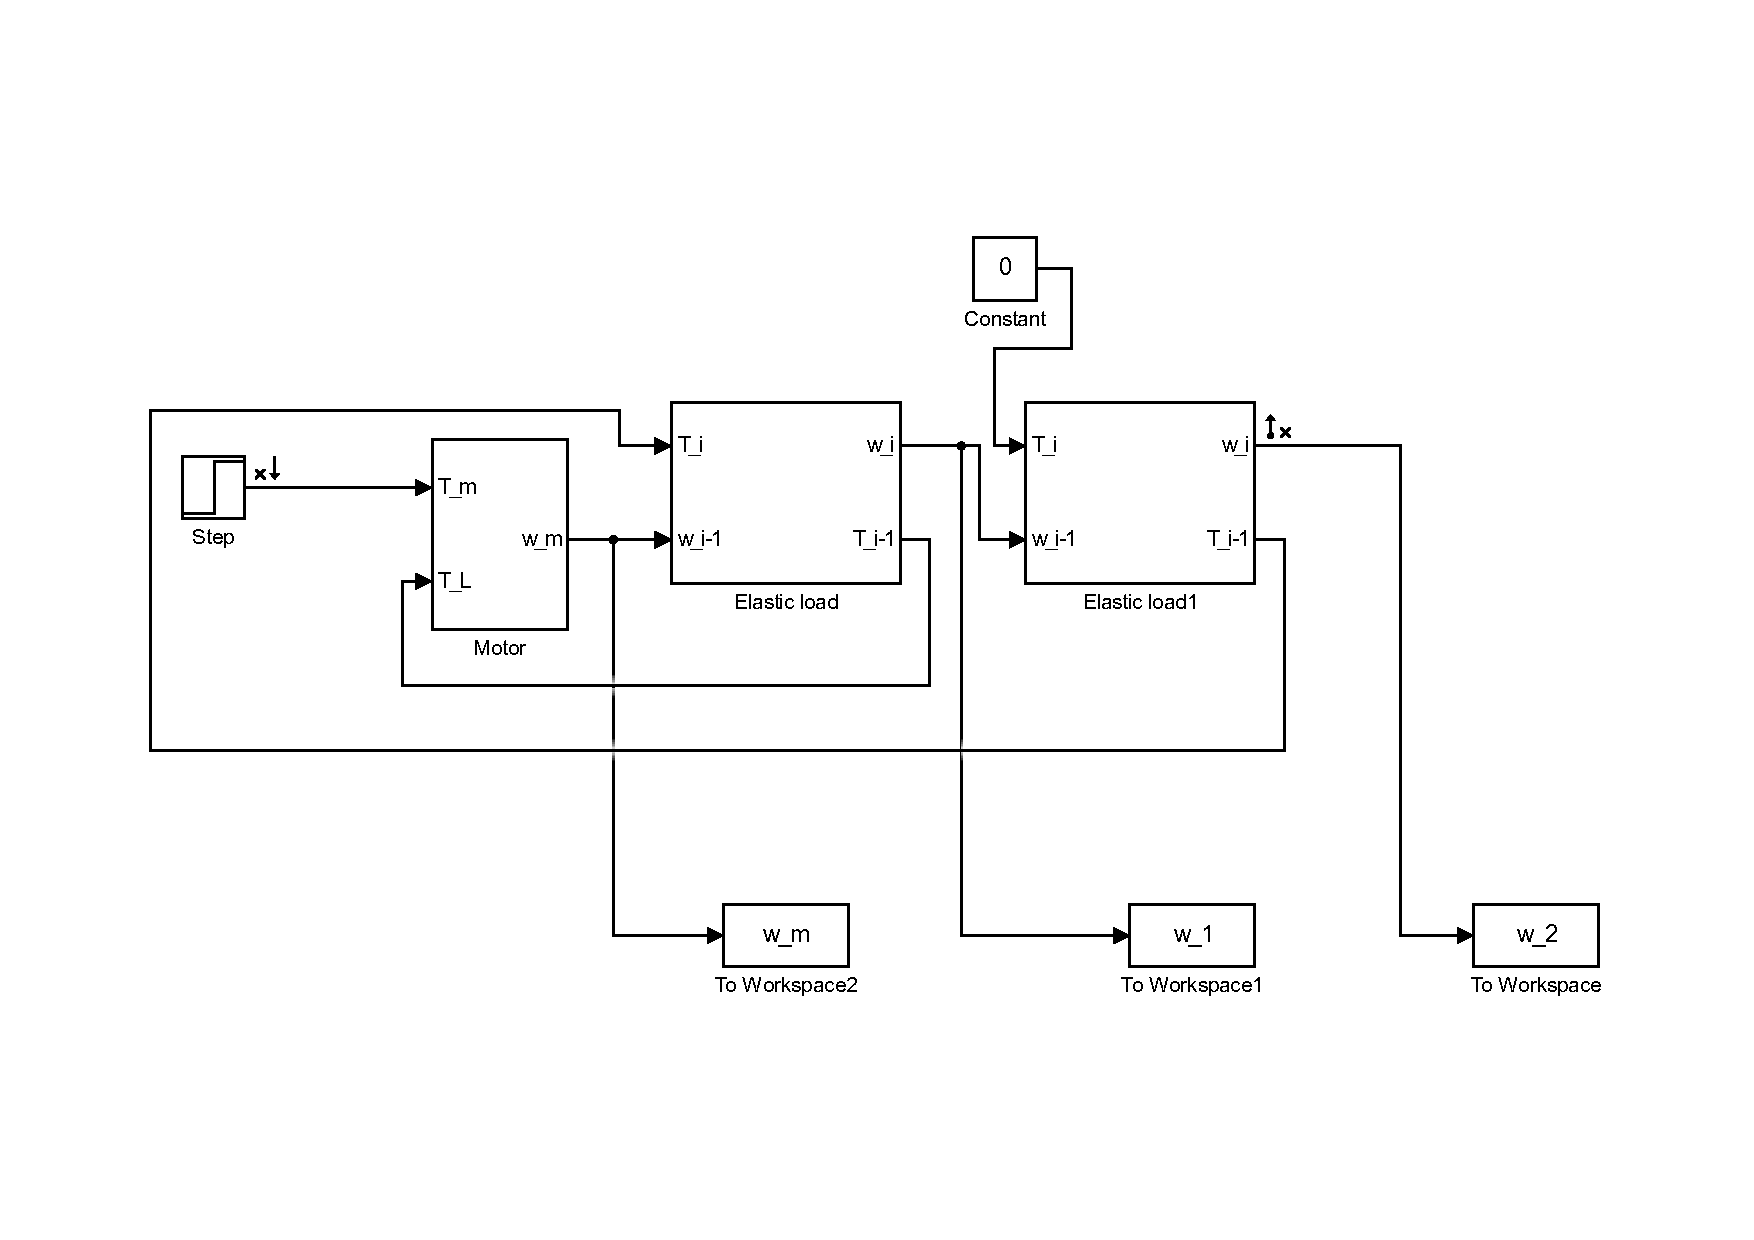
\includegraphics[width = \textwidth]{ex1_2}
    \caption{Two elastc loads in series with the motor.}
    \label{fig:twoloads} 
\end{figure}

\begin{figure}[!ht]
    \centering
    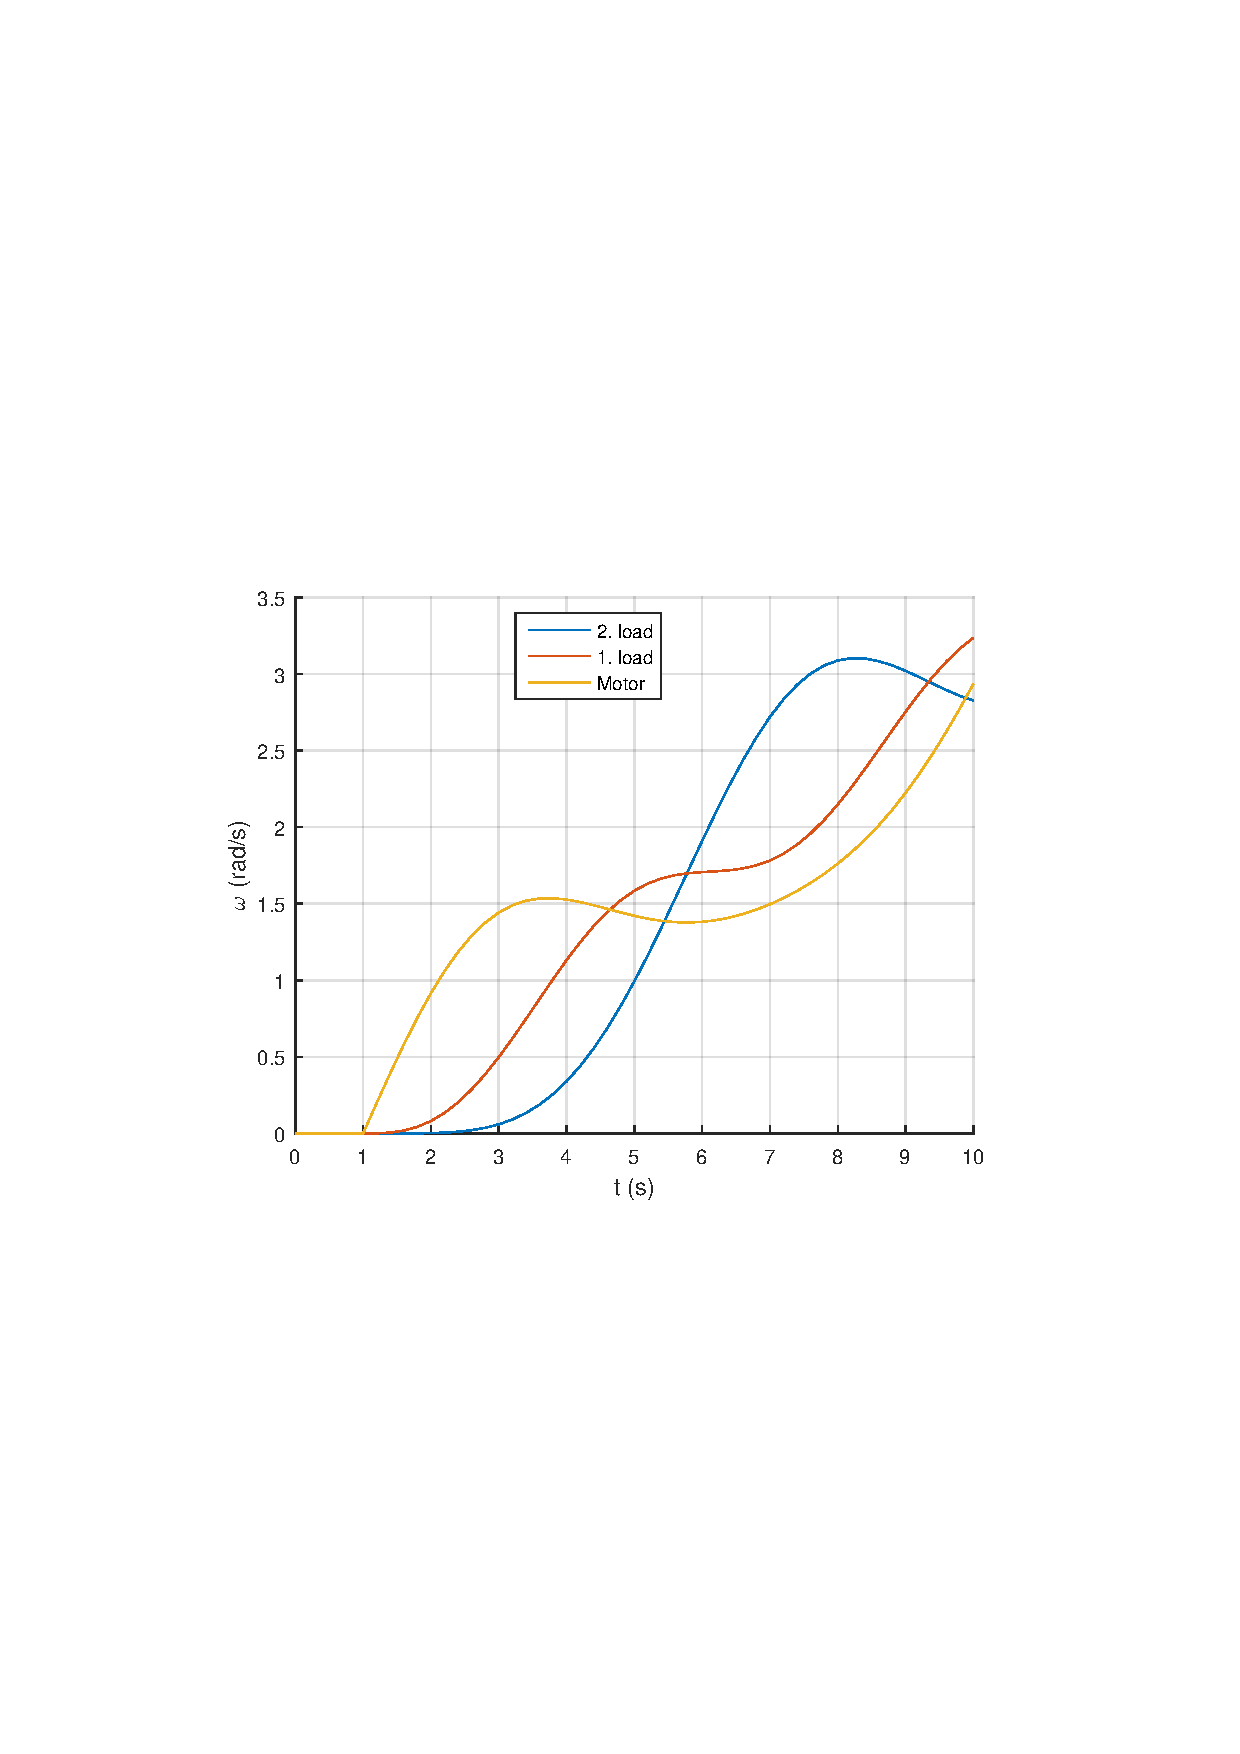
\includegraphics[width = \textwidth]{ex1_2b}
    \caption{Plot of the rotational velocity of the motor and the two loads.}
    \label{fig:veloplot} 
\end{figure}

As seen in Figure \ref{fig:veloplot}, the angular velocity of the second load is greatly amplified. It is also delayed by a couple of seconds, which is natural to except of this system. Otherwise the rotational velocity of the last load behaves quite similary to that of the motor and the fist load.

\subsection{e}

\begin{figure}[!ht]
    \centering
    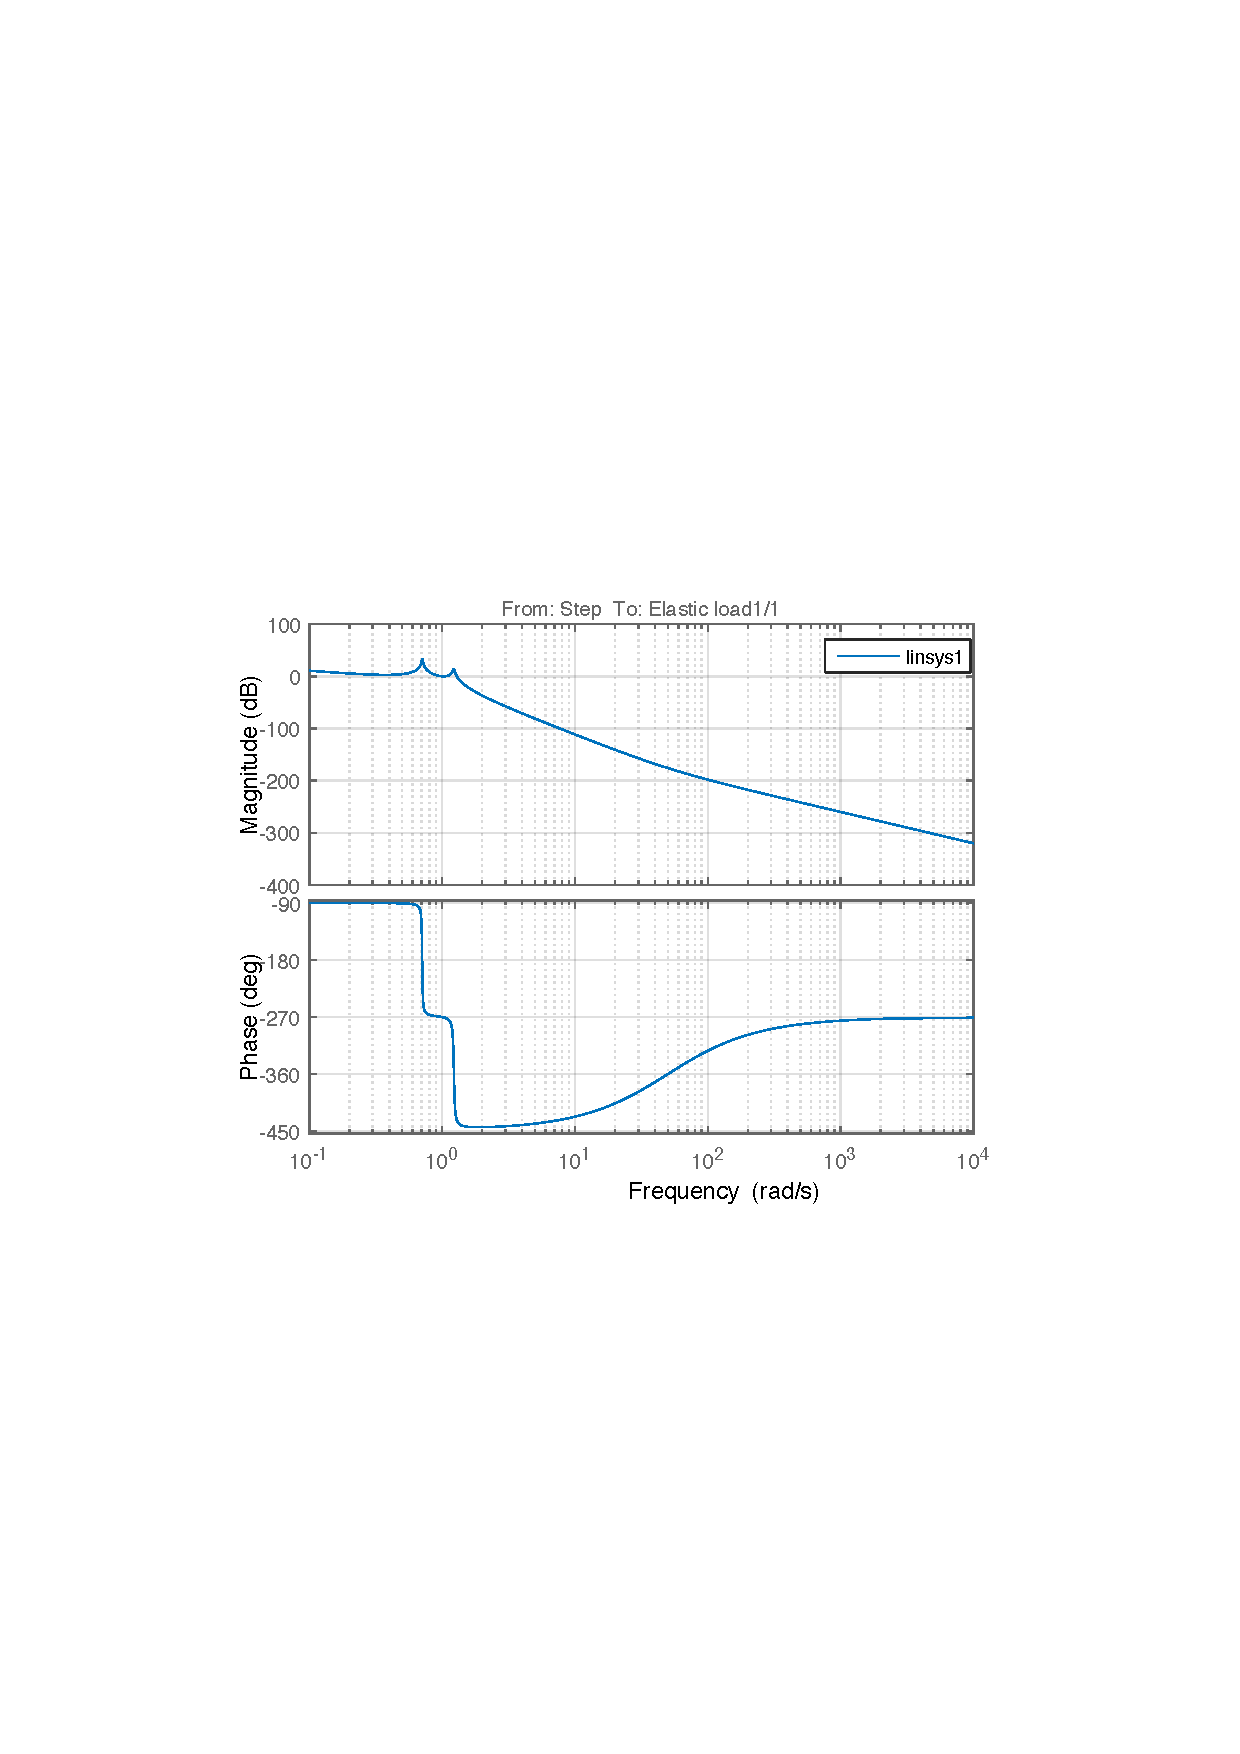
\includegraphics[width = \textwidth]{ex1_2_bode}
    \caption{Bode plot of the transfer function from the step input to the rotational velocity of the second load.}
    \label{fig:bodeSimu} 
\end{figure}

\newpage

\section{Problem 3}

\subsection{a}

\begin{figure}[h]
    \centering
    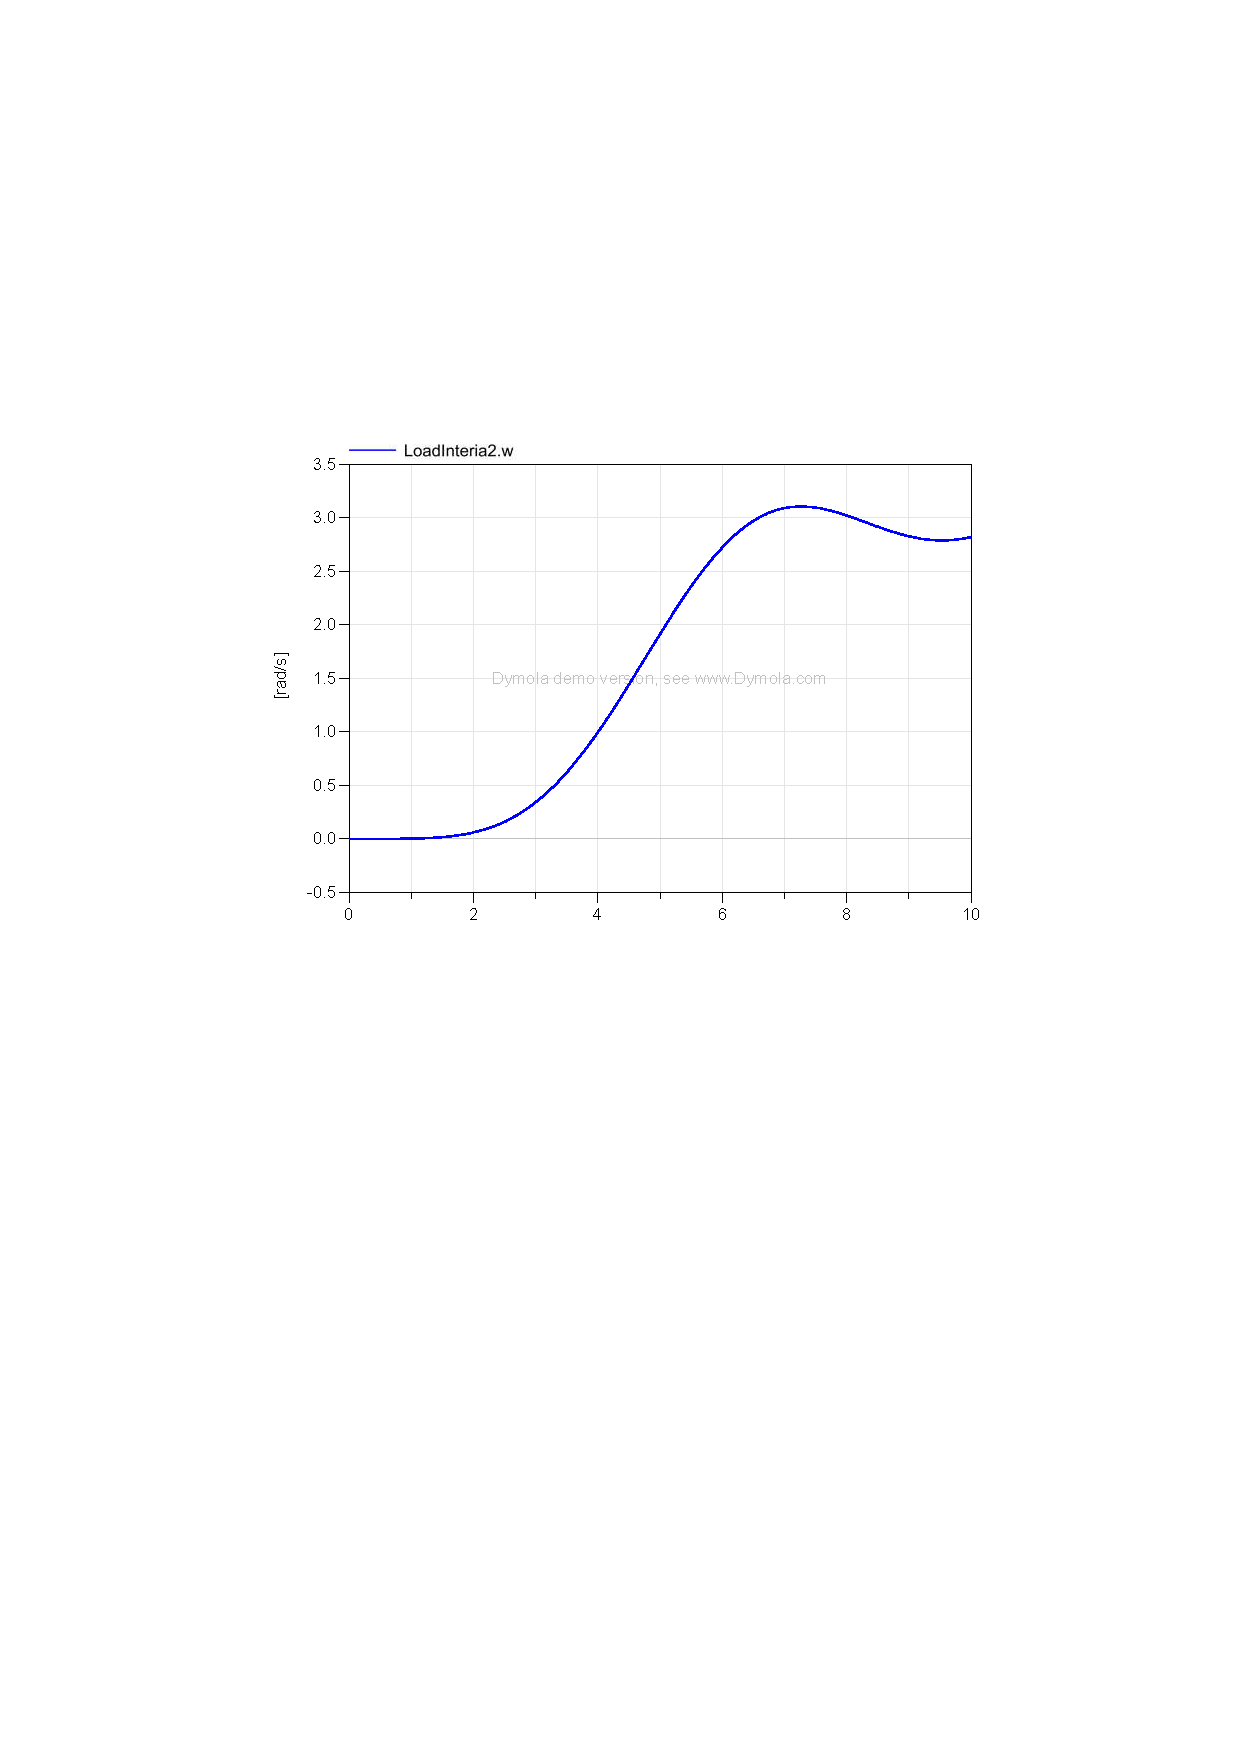
\includegraphics[width = \textwidth]{ex1_3a}
    \caption{The rotational velocity of the second load when simulated using Dymola.}
    \label{fig:dymola1} 
\end{figure}

\subsection{b}

\subsection{c}

\begin{figure}[h]
    \centering
    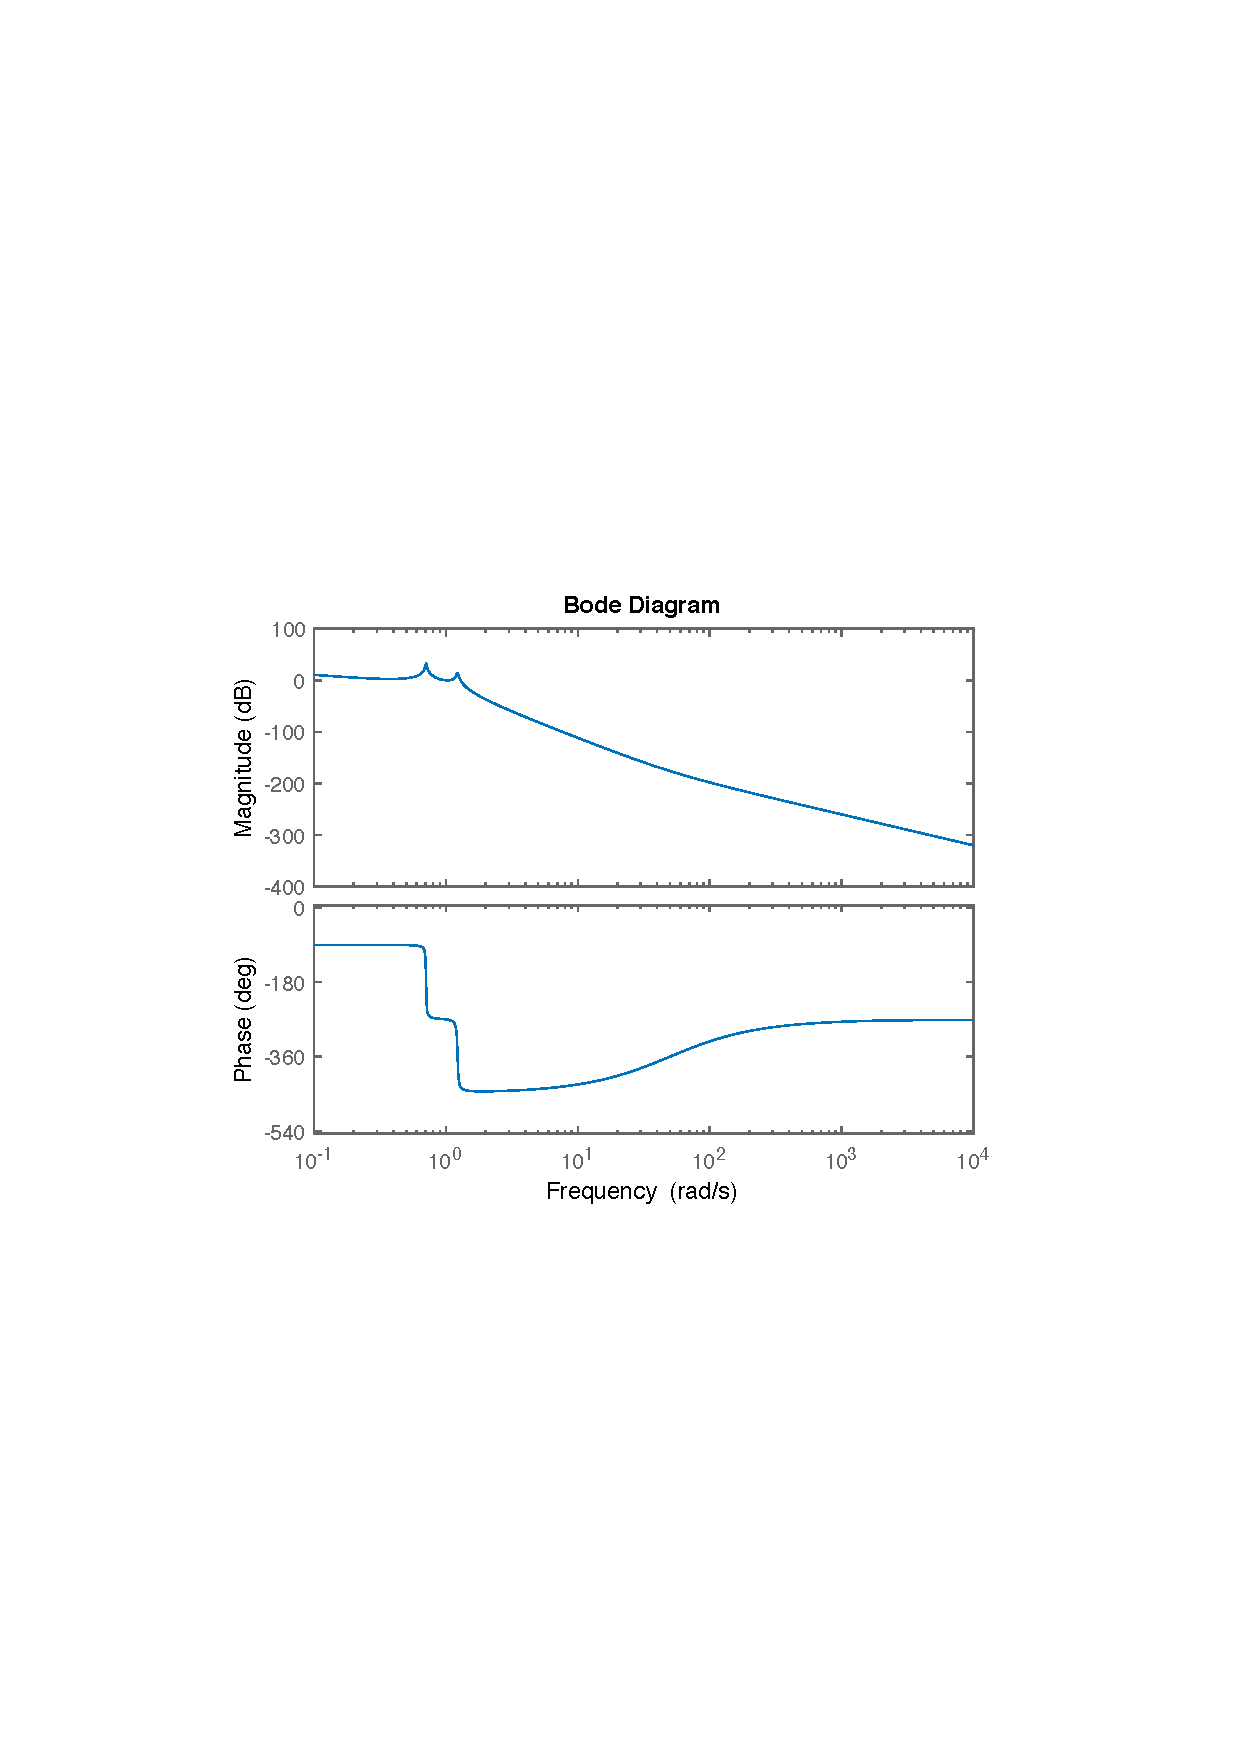
\includegraphics[width = \textwidth]{ex1_3c_bode}
    \caption{Bode plot of the system when linearized with Dymola.}
    \label{fig:bodeDymola} 
\end{figure}



\end{document}